\documentclass{standalone}
\usepackage[T1]{fontenc}
\usepackage[utf8]{inputenc}
\usepackage[usenames,dvipsnames]{xcolor}
\usepackage{tikz}
\usetikzlibrary{plotmarks}
\usetikzlibrary{shapes,snakes,arrows}
\begin{document}
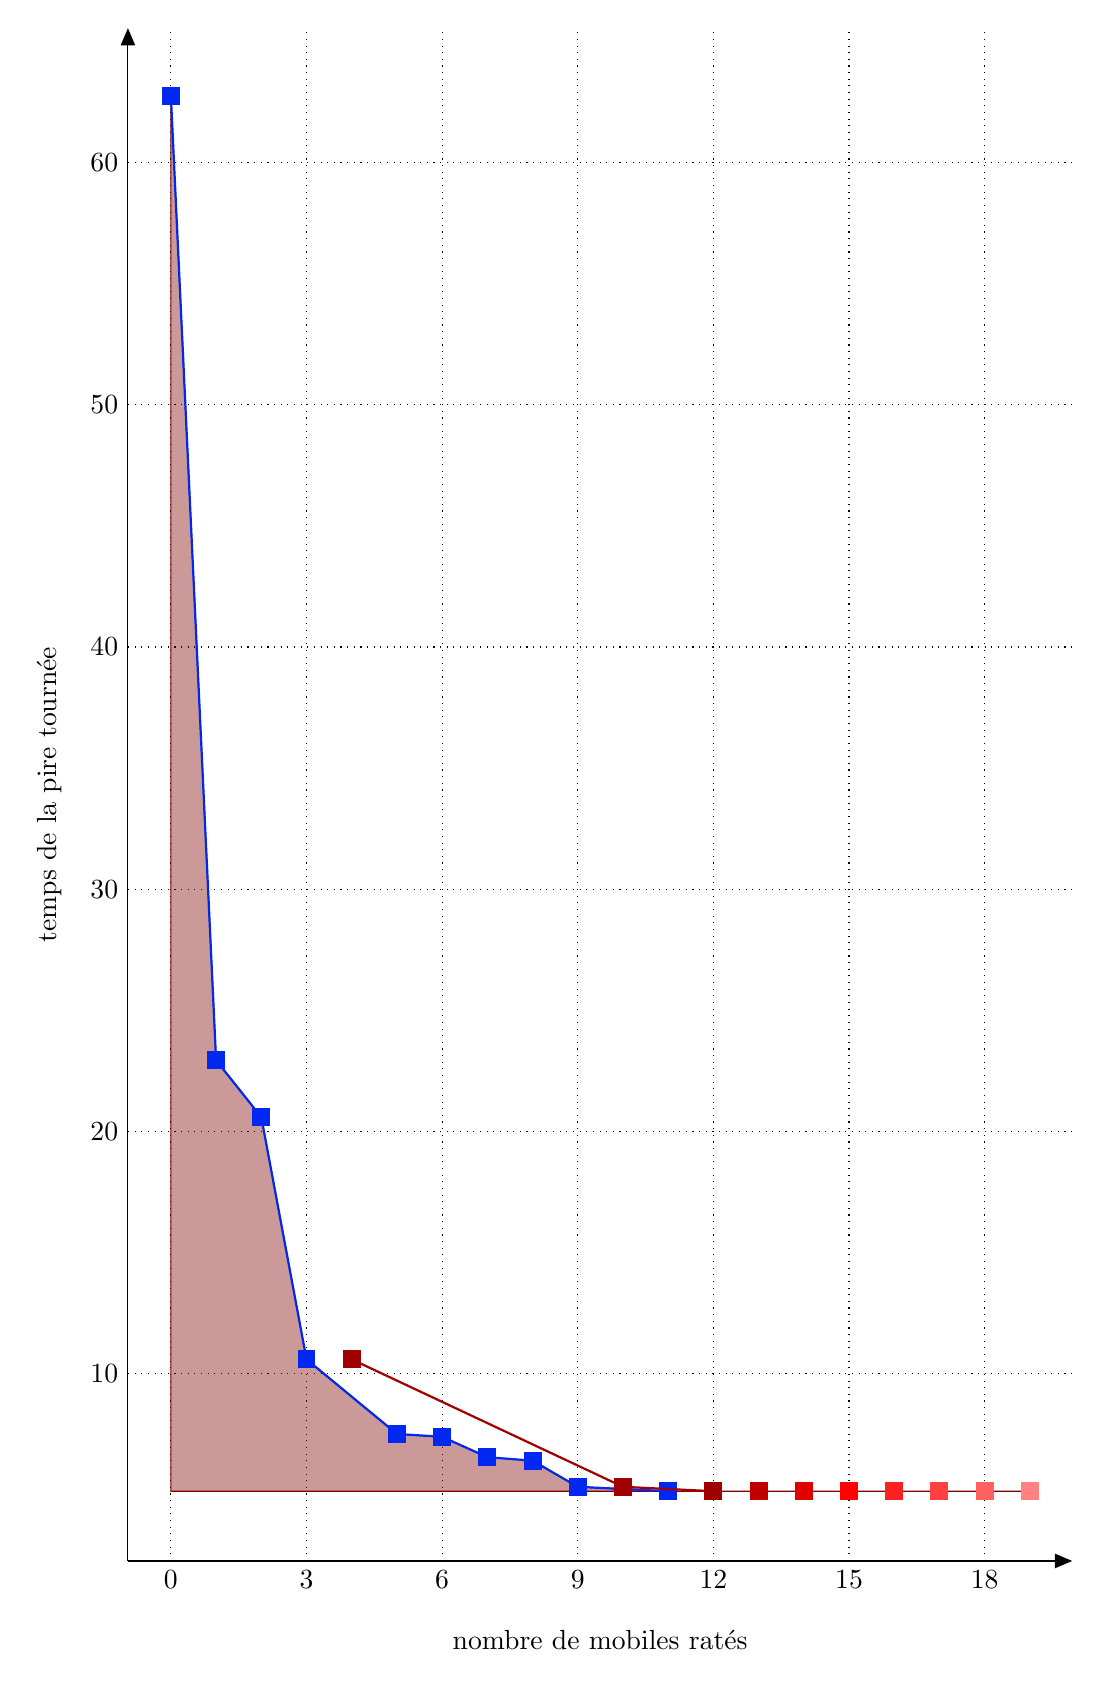
\begin{tikzpicture}[xscale=0.574163,yscale=0.307612]
\draw[xstep=3,ystep=10,thin,dotted,color=Black] (-0.95,2.26929) grid (19.9366,65.5484);
\begin{scope}
  \clip (-0.95,2.26929) rectangle (19.9366,65.5484);
  \definecolor{hvColor}{RGB}{128,0,0}
  \draw[color=hvColor, fill=hvColor, fill opacity=0.4] (0,5.14916) -- (0,62.7466) -- (1,22.94) -- (2,20.59) -- (3,10.592) -- (5,7.51176) -- (6,7.39466) -- (7,6.55359) -- (8,6.40903) -- (9,5.33074) -- (11,5.14916) -| (19,5.14916) -- cycle;
  \definecolor{pLineColor}{RGB}{128,0,0}
  \definecolor{pPointColor}{RGB}{0,40,240}
  \draw[thick,color=pPointColor] (0,62.7466) node[draw,color=pPointColor,fill=pPointColor, inner sep = 0pt, minimum size=2mm] {} -- (1,22.94) node[draw,color=pPointColor,fill=pPointColor, inner sep = 0pt, minimum size=2mm] {} -- (2,20.59) node[draw,color=pPointColor,fill=pPointColor, inner sep = 0pt, minimum size=2mm] {} -- (3,10.592) node[draw,color=pPointColor,fill=pPointColor, inner sep = 0pt, minimum size=2mm] {} -- (5,7.51176) node[draw,color=pPointColor,fill=pPointColor, inner sep = 0pt, minimum size=2mm] {} -- (6,7.39466) node[draw,color=pPointColor,fill=pPointColor, inner sep = 0pt, minimum size=2mm] {} -- (7,6.55359) node[draw,color=pPointColor,fill=pPointColor, inner sep = 0pt, minimum size=2mm] {} -- (8,6.40903) node[draw,color=pPointColor,fill=pPointColor, inner sep = 0pt, minimum size=2mm] {} -- (9,5.33074) node[draw,color=pPointColor,fill=pPointColor, inner sep = 0pt, minimum size=2mm] {} -- (11,5.14916) node[draw,color=pPointColor,fill=pPointColor, inner sep = 0pt, minimum size=2mm] {};
  \definecolor{pLineColor}{RGB}{160,0,0}
  \definecolor{pPointColor}{RGB}{160,0,0}
  \draw[thick,color=pPointColor] (4,10.592) node[draw,color=pPointColor,fill=pPointColor, inner sep = 0pt, minimum size=2mm] {} -- (10,5.33074) node[draw,color=pPointColor,fill=pPointColor, inner sep = 0pt, minimum size=2mm] {} -- (12,5.14916) node[draw,color=pPointColor,fill=pPointColor, inner sep = 0pt, minimum size=2mm] {};
  \definecolor{pLineColor}{RGB}{192,0,0}
  \definecolor{pPointColor}{RGB}{192,0,0}
  \draw[thick,color=pPointColor] (13,5.14916) node[draw,color=pPointColor,fill=pPointColor, inner sep = 0pt, minimum size=2mm] {};
  \definecolor{pLineColor}{RGB}{224,0,0}
  \definecolor{pPointColor}{RGB}{224,0,0}
  \draw[thick,color=pPointColor] (14,5.14916) node[draw,color=pPointColor,fill=pPointColor, inner sep = 0pt, minimum size=2mm] {};
  \definecolor{pLineColor}{RGB}{255,1,1}
  \definecolor{pPointColor}{RGB}{255,1,1}
  \draw[thick,color=pPointColor] (15,5.14916) node[draw,color=pPointColor,fill=pPointColor, inner sep = 0pt, minimum size=2mm] {};
  \definecolor{pLineColor}{RGB}{255,33,33}
  \definecolor{pPointColor}{RGB}{255,33,33}
  \draw[thick,color=pPointColor] (16,5.14916) node[draw,color=pPointColor,fill=pPointColor, inner sep = 0pt, minimum size=2mm] {};
  \definecolor{pLineColor}{RGB}{255,65,65}
  \definecolor{pPointColor}{RGB}{255,65,65}
  \draw[thick,color=pPointColor] (17,5.14916) node[draw,color=pPointColor,fill=pPointColor, inner sep = 0pt, minimum size=2mm] {};
  \definecolor{pLineColor}{RGB}{255,97,97}
  \definecolor{pPointColor}{RGB}{255,97,97}
  \draw[thick,color=pPointColor] (18,5.14916) node[draw,color=pPointColor,fill=pPointColor, inner sep = 0pt, minimum size=2mm] {};
  \definecolor{pLineColor}{RGB}{255,129,129}
  \definecolor{pPointColor}{RGB}{255,129,129}
  \draw[thick,color=pPointColor] (19,5.14916) node[draw,color=pPointColor,fill=pPointColor, inner sep = 0pt, minimum size=2mm] {};
\end{scope}
\draw[->,>=triangle 45] (-0.95,2.26929) -- coordinate (x axis mid) (19.9366,2.26929);
\node[below=1cm,anchor=center] at (x axis mid) {nombre de mobiles ratés};
\foreach \x in {0,3,6,9,12,15,18}
  \draw (\x,2.26929) -- (\x,2.26929) node[anchor=north] {\x};
\draw[->,>=triangle 45] (-0.95,2.26929) -- coordinate (y axis mid) (-0.95,65.5484);
\node[left=1cm,rotate=90,anchor=center] at (y axis mid) {temps de la pire tournée};
\foreach \y in {10,20,30,40,50,60}
  \draw (-0.95,\y) -- (-0.95,\y) node[anchor=east] {\y};
\end{tikzpicture}
\end{document}
